%%%%%%%%%%%%%%%%%%%%%%%%%%%%%%%%%%%%%%%%%%%%%%%%%%%%%%%%%%%%%%%%%%%%%%%%%%%%%%%%%%%%%%%
%%%%%%%%%%%%%%%%%%%%%%%%%%%%%%%%%%%%%%%%%%%%%%%%%%%%%%%%%%%%%%%%%%%%%%%%%%%%%%%%%%%%%%%
% 
% This top part of the document is called the 'preamble'.  Modify it with caution!
%
% The real document starts below where it says 'The main document starts here'.

\documentclass[12pt]{article}

\usepackage{amssymb,amsmath,amsthm}
\usepackage[top=1in, bottom=1in, left=1.25in, right=1.25in]{geometry}
\usepackage{fancyhdr}
\usepackage{graphicx}
\usepackage{enumerate}
\usepackage{verbatim}
\usepackage{listings}
\usepackage{float}

% Comment the following line to use TeX's default font of Computer Modern.
\usepackage{times,txfonts}

\newtheoremstyle{homework}% name of the style to be used
  {18pt}% measure of space to leave above the theorem. E.g.: 3pt
  {12pt}% measure of space to leave below the theorem. E.g.: 3pt
  {}% name of font to use in the body of the theorem
  {}% measure of space to indent
  {\bfseries}% name of head font
  {:}% punctuation between head and body
  {2ex}% space after theorem head; " " = normal interword space
  {}% Manually specify head
\theoremstyle{homework} 

% Set up an Exercise environment and a Solution label.
\newtheorem*{exercisecore}{\@currentlabel}
\newenvironment{exercise}[1]
{\def\@currentlabel{#1}\exercisecore}
{\endexercisecore}

\newcommand{\localhead}[1]{\par\smallskip\noindent\textbf{#1}\nobreak\\}%
\newcommand\solution{\localhead{Solution:}}



% \newcommand{includematlab}[1]{\verbatiminput{#1}}

%%%%%%%%%%%%%%%%%%%%%%%%%%%%%%%%%%%%%%%%%%%%%%%%%%%%%%%%%%%%%%%%%%%%%%%%
%
% Stuff for getting the name/document date/title across the header
\makeatletter
\RequirePackage{fancyhdr}
\pagestyle{fancy}
\fancyfoot[C]{\ifnum \value{page} > 1\relax\thepage\fi}
\fancyhead[L]{\ifx\@doclabel\@empty\else\@doclabel\fi}
\fancyhead[C]{\ifx\@docdate\@empty\else\@docdate\fi}
\fancyhead[R]{\ifx\@docauthor\@empty\else\@docauthor\fi}
\headheight 15pt

\def\doclabel#1{\gdef\@doclabel{#1}}
\doclabel{Use {\tt\textbackslash doclabel\{MY LABEL\}}.}
\def\docdate#1{\gdef\@docdate{#1}}
\docdate{Use {\tt\textbackslash docdate\{MY DATE\}}.}
\def\docauthor#1{\gdef\@docauthor{#1}}
\docauthor{Use {\tt\textbackslash docauthor\{MY NAME\}}.}
\makeatother

%% General formatting parameters
\parindent 0pt
\parskip 12pt plus 1pt

\def\vx{\mathbf x}
\def\vb{\mathbf b}

% Shortcuts for blackboard bold number sets (reals, integers, etc.)
\newcommand{\Reals}{\ensuremath{\mathbb R}}
\newcommand{\Nats}{\ensuremath{\mathbb N}}
\newcommand{\Ints}{\ensuremath{\mathbb Z}}
\newcommand{\Rats}{\ensuremath{\mathbb Q}}
\newcommand{\Cplx}{\ensuremath{\mathbb C}}
%% Some equivalents that some people may prefer.
\let\RR\Reals
\let\NN\Nats
\let\II\Ints
\let\CC\Cplx

%%%%%%%%%%%%%%%%%%%%%%%%%%%%%%%%%%%%%%%%%%%%%%%%%%%%%%%%%%%%%%%%%%%%%%%%%%%%%%%%%%%%%%%
%%%%%%%%%%%%%%%%%%%%%%%%%%%%%%%%%%%%%%%%%%%%%%%%%%%%%%%%%%%%%%%%%%%%%%%%%%%%%%%%%%%%%%%
% 
% The main document start here.

% The following commands set up the material that appears in the header.

%%%%%%%%%%%%%%%%%%%%%%%%%%%%%%%%%%%%%%%%%%%%%%%%%%%%%%%%%%%%%%%%%%%%%%%%%%
\doclabel{Math 426: Homework 11}
\docauthor{Stefano Fochesatto}
\docdate{November 11, 2020}

\begin{document}

\begin{exercise}{Supplemental 1}
Find $n$ so that degree $n$ polynomial interpolation of 
$f(x)=\cos(3x)$, using equally-spaced points on $[0, 2]$, gives a maximum approximation error $|f(x) - p(x)|$ which is less than $10^{-6}$ on 
$[0, 2]$. 

Then use MATLAB's polyfit and polyval and a bit of trial and error
to find the actual smallest $n$ needed 
to approximate $f(x) = \cos(3x)$ to within $10^{-6}$.\\

\solution In class we demonstrated that given $f$ is $n+1$ times differentiable on $[a,b]$, $x_0,\dots,x_n$ then there exists an $\xi \in [a,b]$ the error of an $n$ degree polynomial interpolant,
\begin{equation*}
  |f(x) - p(x)| = f^{(n+1)}(\xi)\dfrac{\prod_{k = 0}^n (x - x_k)}{(n+1)!}
\end{equation*} 
Finding $n$ so that the maximum error term of $p(x)$ on the interval $[0,2]$ is less than $10^{-6}$,
\begin{equation*}
  f^{(n+1)}(\xi)\dfrac{\prod_{k = 0}^n (x - x_k)}{(n+1)!} \le 10^{-6}.
\end{equation*} 
Note that, when differentiate $cos(3x)$, $n+1$ times we get a trig function whose maximum value is $1$ multiplied by $3^{n+1}$ so,
\begin{equation*}
  3^{n+1}\dfrac{\prod_{k = 0}^n (x - x_k)}{(n+1)!} \le 10^{-6}.
\end{equation*} 
Also note that the maximum size of each term in the product is 2 so,
\begin{equation*}
  3^{n+1}\dfrac{2^{n+1}}{(n+1)!} \le 10^{-6}.
\end{equation*} 
Using MATLAB we get that when $n\geq 25$ then this statement is true. \\

Using MATLAB's polyfit and polyval approximate to approximate $n$ by trial and error we get $n \geq 13$,\\
\textbf{Function:}
\begin{center}
\lstinputlisting{HW11_Sup.m}
\end{center}

\textbf{Console:}
\begin{center}
\lstinputlisting{Sup1console.txt}
\end{center}
\end{exercise}
\vspace{.5in}





\begin{exercise}{Text 8.9} Determine the piecewise polynomial function,
  \begin{equation*}
    P(x) = 
    \begin{cases} 
      P_1(x) & 0\leq x \leq 1, \\
      P_2(x) & 1\leq x\leq 2, 
   \end{cases}
  \end{equation*}
  That is defined by the following conditions,
  \begin{enumerate}
    \item $P_1(x)$ is linear.
    \item $P_2(x)$ is quadratic.
    \item $P(x)$ and $P'(x)$ are continuous at $x = 1$.
    \item $P(0) = 1$, $P(1) = -1$, and $P(2) = 0$.
  \end{enumerate}
  Plot the function. \\
  \solution Note that since $P(0) = 1$, $P(1) = -1$ and $P_1(x)$ is linear we know that 
  \begin{equation*}
    P_1(x) = -2x+1.
  \end{equation*}
  Since $P_2(x)$ is a quadratic we know it is of the following form,
  \begin{equation*}
    P_2(x) = c_2x^2 + c_1x + c_0.
  \end{equation*}
  Since $P(2) = 0$ we get the following equation,
  \begin{equation*}
    0 = c_2(2)^2 + c_1(2) + c_0.
  \end{equation*}
  and since $P(x)$ and $P'(x)$ are continuous at $x = 1$ we get that
  \begin{equation*}
    -1 = c_2(1)^2 + c_1(1) + c_0.
  \end{equation*}
  \begin{equation*}
    -2 = c_2(2)(1) + c_1 + (0)c_0.
  \end{equation*}
  Solving the system of equations(lazily with MATLAB) we get that
  \begin{equation*}
    P_2(x) = 3x^2  - 8x + 4.
  \end{equation*}
  Finally, all together we see that,
  \begin{equation*}
    P(x) = 
    \begin{cases} 
      -2x+1 & 0\leq x \leq 1, \\
      3x^2  - 8x + 4 & 1\leq x\leq 2, 
   \end{cases}
  \end{equation*}
\end{exercise}
\vspace{.5in}






\begin{exercise}{Text 8.7 (a,b)} Use MATLAB to  various piecewise polynomials to  the  Runge function, using the same nodes as in part(a) of exercise 4.\\
  \begin{enumerate}
    \item Find the piecewise linear interpolant of $f(x)$.  (You  may useMATLAB routine interp1 or write your own routine.)\\
    \solution 
    \textbf{Console:}
    \begin{center}
    \lstinputlisting{HW87.txt}
    \end{center}
    \begin{figure}[H]
      \caption{Plot of linear interpolation for the Runge function with 13 sample points}
      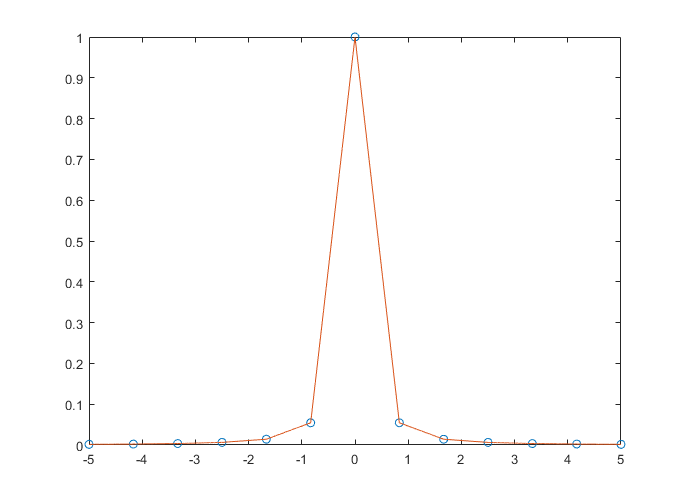
\includegraphics[width = \textwidth]{linear_interRunge.png}  
      \centering
   \end{figure}
   \vspace{.25in}

   \item Find the piecewise cubic Hermite interpolant of $f(x)$. (Write your own routine for this, using formulas (8.17) and (8.18).)\\
   \solution

   
   \textbf{Function:}
   \begin{center}
   \lstinputlisting{cubicHermite.m}
   \end{center}
   
   
   
   \textbf{Console:}
    \begin{center}
    \lstinputlisting{Hermmite.txt}
    \end{center}
  
    \begin{figure}[H]
      \caption{Plot of cubicHermite interpolation for the Runge function with 13 sample points}
      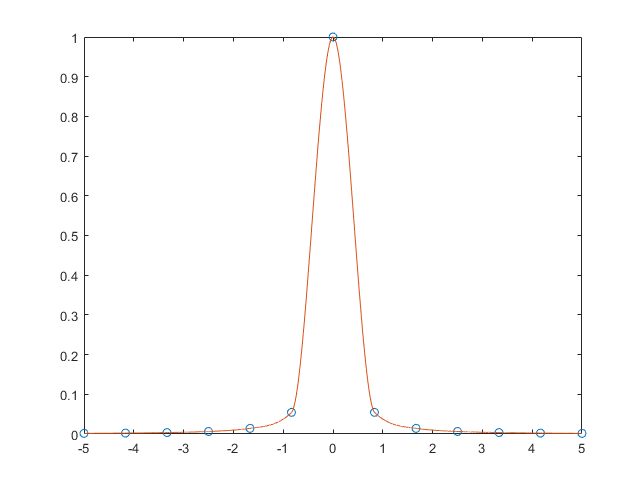
\includegraphics[width = \textwidth]{cubichermite.png}  
      \centering
   \end{figure}



  
  
  \end{enumerate}






\end{exercise}
\vspace{.5in}















\begin{exercise}{Text 8.8} Computer libraries often use tables of function values together with piecewise linear interpolation to evaluate elementary functions such as $sin x$, 
  because table lookup and interpolation can be faster than, say,using a Taylor series expansion.\\
  \begin{enumerate}
    \item In MATLAB create a $x$ of 1000 uniformly ­spaced values between 0 and $\pi$ . 
    Then create a vector $y$ with the values of the sine function at each of these points.\\
    \textbf{Console:}
    \begin{center}
    \lstinputlisting{setup.txt}
    \end{center}
    

    \vspace{.25in}
    \item Next create a vector $r$ of 100 randomly distributed values between 0  and $\pi$.  (This  can  be  done in  MATLAB by  typing $r  =  pirand(100,1);$.) Estimate $sin(r)$  
    as  follows: For  each value $r(j)$,find the two consecutive 
    $x$ entries, $x(i)$ and $x(i+1)$ that satisfy $x(i) \le r(j) \le x(i+1)$.  Having  identified  the  
    sub-interval that  contains $r(j)$, use linear interpolation to estimate $sin(r(j))$. Compare your results with those returned 
    by MATLAB when you type $sin(r)$. Find the maximum absolute error and the maximum relative error in your results.\\
    \textbf{Console:}
    \begin{center}
    \lstinputlisting{LinearInterpolation_estimate.txt}
    \end{center}

    \textbf{Function HW88:}
    \begin{center}
    \lstinputlisting{HW88.m}
    \end{center}

    \begin{figure}[H]
      \caption{Plot of linear interpolation with $x$ sample points}
      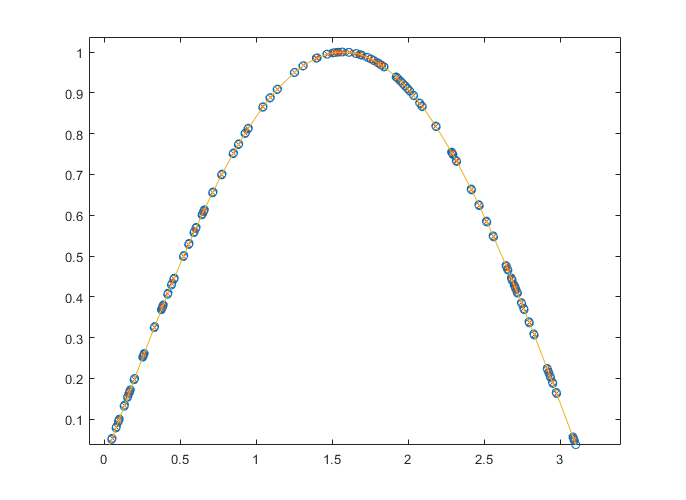
\includegraphics[width = .80\textwidth]{linear_interpolation.png}  
      \centering
   \end{figure}

   \begin{figure}[H]
    \caption{Linear interpolation zoomed in, O are sample points, $x$ are $sin(r(j))$ approximation}
    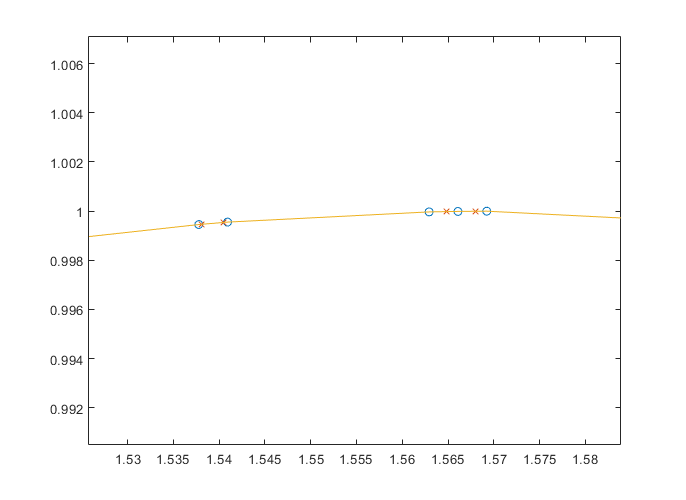
\includegraphics[width = .80\textwidth]{linear_interpolation_zoom.png}  
    \centering
 \end{figure}
  \end{enumerate}
\end{exercise}
\vspace{.5in}














\begin{exercise}{Supplemental 2}
At the bottom of page 198 is an inequality that describes the error from the piecewise-linear interpolant $\ell(x)$ for $f(x)$ on $[a, b]$. Suppose we have equally spaced points $a=x_0 <x_1 <\cdots<x_n =b$ with spacing
$h=x_i-x_{i-1}$. Then:
\[
|f(x)-\ell(x)|\le\frac{Mh^2}{8}
\]
for all $x\in[a,b]$.
In this inequality we are assuming $f''(x)$ exists and is bounded by the number $M$, so that $|f''(x)| \le M$ for all $x \in [a,b]$.
Use this inequality  to find $n$ so that $|f(x)-l(x)| \le 10^{-6}$
for $x \in [0,2] $ if $f(x) = \cos(3x)$.\\
\solution Note that with evenly spaced points the value for $h = \frac{b - a}{n}$. Therefore we seek to solve the inequality,
\begin{equation*}
  \dfrac{M(\frac{2}{n})^2}{8} \le 10^{-6}.
\end{equation*} 
Note that the second derivative of $f(x) = cos(3x)$, is $f''(x) = -9cos(3x)$. Since $|cos(3x)|\le 1$ we know that $M = 9$. Solving the inequality for $n$,
\begin{align*}
  \dfrac{9(\frac{2}{n})^2}{8} &\le 10^{-6},\\
  \dfrac{36}{8n^2} &\le 10^{-6},\\
  \sqrt{\dfrac{36 * 10^{6}}{8}} &\le n,\\
  2122 &\le n.
\end{align*}






\end{exercise}

\end{document}